\documentclass[12pt,fleqn]{article}\usepackage{../../common}
\begin{document}
Uygulama - Yağmur Yağış Verisi

Yağış verisini nasıl analiz ederiz? Bir örnek üzerinde görelim, [1]'den alınan
Singapur yağış verisi,

\begin{minted}[fontsize=\footnotesize]{python}
import pandas as pd
df = pd.read_csv('rainfall.csv',index_col=0,parse_dates=['dt'])
df.columns = ['rain']
print (df)
\end{minted}

\begin{verbatim}
            rain
dt              
2015-01-01   0.6
2015-01-02   0.0
2015-01-03   0.0
2015-01-04   0.0
2015-01-05   0.0
...          ...
2022-01-27   0.0
2022-01-28   0.0
2022-01-29   0.0
2022-01-30   3.8
2022-01-31   0.0

[2588 rows x 1 columns]
\end{verbatim}

Yağış verisi milimetre yağış miktarı olarak gösterilmiş. Bazı günlerde hiç yağış
yok, sıfır milimetre su.

Bu verinin dağılımını görmek ilginç olabilir. Tabii her ayın yağış dağılımı
farklı olabilir, mesela altta Mart ayına bakalım,

\begin{minted}[fontsize=\footnotesize]{python}
x = df[df.index.month == 3]['rain']
\end{minted}

Bu veriye ne tür dağılım uygun olur? Literatürde pek çok kullanım var.  Bazıları
Gamma, bazıları Weibull diyor. Biz altta ikisini de test edeceğiz.

\begin{minted}[fontsize=\footnotesize]{python}
from scipy.stats import gamma
res = gamma.fit(df['rain'])
a,loc,scale = res  
x.hist(density=True)
plt.ylim(0,0.4)
plt.plot(x, gamma.pdf(x,a,loc,scale),'r.')
plt.savefig('stat_176_app1_01.png')
\end{minted}

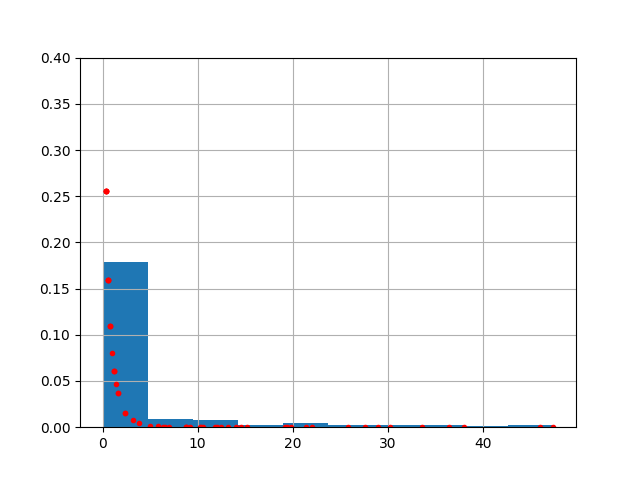
\includegraphics[width=20em]{stat_176_app1_01.png}

Hem veriden gelen histogramı hem de olasılık yoğunluk fonksiyonunu aynı
grafikte gösterdik, kabaca ilk kontrol bu şekilde yapılabilir.

Daha detayli veriye olan uygunluğu kontrol için olasılık dağılımları arasında
bir yakınlık ölçüsü olan Kullback-Leibler mesafesini [2] kullanalım. Veri
histogramı ve tahmin edilen dağılım üzerinden üretilenlerin histogramı arasında
mesafeyi alttaki fonksiyon ile ölçebiliriz,

\begin{minted}[fontsize=\footnotesize]{python}
def kl(p, q):
    return np.sum(p * np.log(p / q))    
\end{minted}

\begin{minted}[fontsize=\footnotesize]{python}
b = range(0,50)
eps = 1e-5
s = 4000
dh = np.histogram(df.rain, bins=b, density=True)[0]+eps

r1 = gamma.rvs(a,loc,scale,size=s)
h1 = np.histogram(r1, bins=b, density=True)[0]+eps
print ('Gamma', kl(h1, dh))
\end{minted}

\begin{verbatim}
Gamma 0.28355078534621225
\end{verbatim}

Weibull Min adlı dağılım için de kontrol yapalım.

\begin{minted}[fontsize=\footnotesize]{python}
from scipy.stats import weibull_min
res = weibull_min.fit(df['rain'])
a,loc,scale = res  
x.hist(density=True)
plt.ylim(0,0.4)
plt.plot(x, weibull_min.pdf(x,a,loc,scale),'r.')
plt.savefig('stat_176_app1_02.png')
\end{minted}

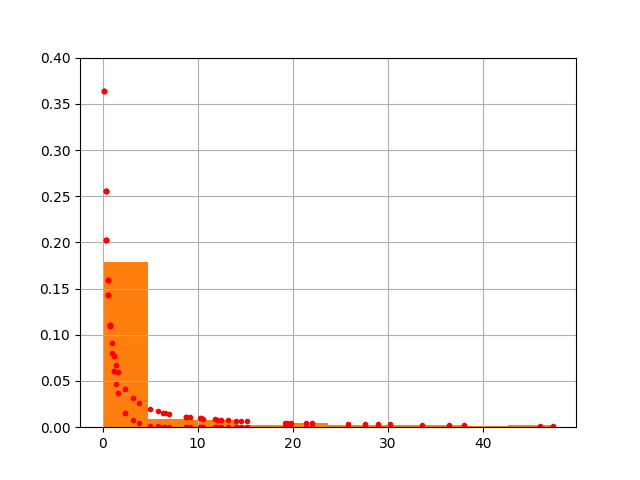
\includegraphics[width=20em]{stat_176_app1_02.png}

\begin{minted}[fontsize=\footnotesize]{python}
r2 = weibull_min.rvs(a,loc,scale,size=s)
h2 = np.histogram(r2, bins=b, density=True)[0]+eps
print ('Weibull Min', kl(h2, dh))
\end{minted}

\begin{verbatim}
Weibull Min 0.06455219814752436
\end{verbatim}

Weibull Min daha yakın gözüküyor.

Yağmur Günleri, Kuraklık Günleri

Bazı araştırmalar ne kadar yağdığını ayrı bir şekilde temsil edip, yagıp
yağmadığı aksiyonunu ayrı bir şekilde tahmin ediyor (bu durumda herhalde miktar
dağılımlarını sadece sıfırdan büyük değerler için kullanmak yeterli
olur). Aksiyon derken ne kadar yağarsa yağsın o gün 'yağdı' olarak alınıyor,
tersi ise 'yağmadı'. Bu ayrıksal konumlar arasındaki geçişler, olasılıksal
şekilde Markov Zincirleri ile temsil edilebilir, bkz [4]'te gösterilen tek gün
öncesine dayanarak yapılan tahmin (ilk örnek). Örnek tek gün öncesini
kullanmış. Fakat önceki iki günün tüm kombinasyonları yağma/yağmama üzerinden 4
konum ile temsil edilirse, o zaman iki gün öncesi de hesaba dahil edilebilir.

Markov Zinciri hazırlığı, önceki gün yağış olup olmadığı D1, iki gün öncesi D2,
bugün D0. 

\begin{minted}[fontsize=\footnotesize]{python}
df = pd.read_csv('rainfall.csv',index_col=0,parse_dates=['dt'])
df.columns = ['rain']
df['r1ago'] = df.rain.shift(1)
df['r2ago'] = df.rain.shift(2)
df['D1'] = df.apply(lambda row: (row.r1ago > 0.0).astype(int), axis=1)
df['D2'] = df.apply(lambda row: (row.r2ago > 0.0).astype(int), axis=1)
df['D0'] = df.apply(lambda row: (row.rain > 0.0).astype(int), axis=1)
pd.set_option('display.max_columns', None)
print (df)
\end{minted}

\begin{verbatim}
            rain  r1ago  r2ago  D1  D2  D0
dt                                        
2015-01-01   0.6    NaN    NaN   0   0   1
2015-01-02   0.0    0.6    NaN   1   0   0
2015-01-03   0.0    0.0    0.6   0   1   0
2015-01-04   0.0    0.0    0.0   0   0   0
2015-01-05   0.0    0.0    0.0   0   0   0
...          ...    ...    ...  ..  ..  ..
2022-01-27   0.0    0.0    0.0   0   0   0
2022-01-28   0.0    0.0    0.0   0   0   0
2022-01-29   0.0    0.0    0.0   0   0   0
2022-01-30   3.8    0.0    0.0   0   0   1
2022-01-31   0.0    3.8    0.0   1   0   0

[2588 rows x 6 columns]
\end{verbatim}

\begin{minted}[fontsize=\footnotesize]{python}
g = df.groupby(['D1','D2','D0']).size().reset_index()
print (g)
\end{minted}

\begin{verbatim}
   D1  D2  D0    0
0   0   0   0  633
1   0   0   1  269
2   0   1   0  268
3   0   1   1  228
4   1   0   0  244
5   1   0   1  253
6   1   1   0  253
7   1   1   1  440
\end{verbatim}

Bu sayıları nasıl Markov matrisine çevireceğimizi anlamak için [1, sf. 193].

Konumları etiketlemek için alttakini yapalım,

\begin{minted}[fontsize=\footnotesize]{python}
pivot = g.pivot_table(index=['D1','D2'], columns='D0', aggfunc='mean')
pivot = pivot.reset_index()
print (pivot)
\end{minted}

\begin{verbatim}
   D1 D2    0     
D0          0    1
0   0  0  633  269
1   0  1  268  228
2   1  0  244  253
3   1  1  253  440
\end{verbatim}

Böylece konum 0,1,2,3 elde ettik. İki gün önce ve bir gün önce yağmadı konumu 0,
iki gün önce yağdı bir gün önce yağmadı konum 1, böyle gidiyor. Şimdi dikkat,
buradan bir Markov matrisi çıkartmak için geçiş hedefinde iki kolonlu bir matris
(yağdı,yağmadı) kullanamayız. O durumda matris 4 x 2 boyutunda olurdu, bu bir
Markov matrisi olmaz. Boyutlar 4 x 4 olmalı. Peki o zaman mesela yağdı, yağmadı
konumundan bugün yağdı konumuna nasıl geçeceğiz? Ufak bir numara kullanarak;
yağdı-yağmadı (2 etiketi) konumundan yağmadı-yağdı konumuna (1 etiketi) geçişi
yapacağız. Öyle ya, yağdı, yağmadı konumundan geçiş yaptıktan sonra yeni bir
gündeyiz, artık bir gün öncesi iki gun oncesi oldu, bugün de 'yağdı' durumu var,
gelinen yer yağmadı-yağdı.

Olasılık verisini oluşturalım. Üstteki matristeki toplamları her satırın nihai
toplamı ile bölelim,

\begin{minted}[fontsize=\footnotesize]{python}
MC = np.array(pivot).astype(float)
probs = MC[:,[2,3]] / MC.sum(axis=1).reshape(4,1)
MC[:,[2,3]] = probs
MC = pd.DataFrame(MC)
MC.columns = ['D1','D2','norain','rain']
print (MC)
\end{minted}

\begin{verbatim}
    D1   D2    norain      rain
0  0.0  0.0  0.701774  0.298226
1  0.0  1.0  0.539235  0.458753
2  1.0  0.0  0.489960  0.508032
3  1.0  1.0  0.364029  0.633094
\end{verbatim}

Ufak bir matris olduğu için bu olasılıkları elle gerekli yerlere kodlayabiliriz,

\begin{minted}[fontsize=\footnotesize]{python}
MCfinal = np.zeros((4,4))
MCfinal[0,0] = MC.loc[0]['norain']
MCfinal[0,2] = MC.loc[0]['rain']
MCfinal[1,0] = MC.loc[1]['norain']
MCfinal[1,2] = MC.loc[1]['rain']
MCfinal[2,1] = MC.loc[2]['norain']
MCfinal[2,3] = MC.loc[2]['rain']
MCfinal[3,1] = MC.loc[3]['norain']
MCfinal[3,3] = MC.loc[3]['rain']
print (MCfinal)
\end{minted}

\begin{verbatim}
[[0.70177384 0.         0.29822616 0.        ]
 [0.53923541 0.         0.45875252 0.        ]
 [0.         0.48995984 0.         0.50803213]
 [0.         0.36402878 0.         0.63309353]]
\end{verbatim}

Markov matrisini elde ettik. Artık bu matris üzerinde ek işlemler
yapabiliriz. Daha önce [4]'te bir, iki, hatta daha fazla adım sonrasını MZ ile
tahmin edebilme kabiliyeti işlendi, basit matris çarpımı ile bu
yapılabiliyor. Eğer dün ve iki gün önce yağmur yağdıysa (etiket 3), acaba
önümüzdeki iki gün, üç gün içinde yağmur yağma olasılığı nedir (aynı etiket)?

\begin{minted}[fontsize=\footnotesize]{python}
import numpy.linalg as lin
P2 = lin.matrix_power(MCfinal,2)
print (P2)
print ('')
P3 = lin.matrix_power(MCfinal,3)
print (P3)
\end{minted}

\begin{verbatim}
[[0.49248652 0.14611884 0.20928732 0.15150847]
 [0.3784213  0.22477031 0.16081411 0.23306102]
 [0.2642037  0.18493831 0.22477031 0.32163185]
 [0.19629721 0.23046426 0.16699912 0.40080741]]

[[0.42440661 0.15769583 0.21390475 0.20224372]
 [0.38677028 0.16363337 0.21596908 0.22924815]
 [0.28513653 0.22721167 0.16363337 0.31781358]
 [0.26203074 0.22772829 0.16426702 0.33858949]]
\end{verbatim}

\begin{minted}[fontsize=\footnotesize]{python}
print (MCfinal[3,3])
print (P2[3,3])
print (P3[3,3])
\end{minted}

\begin{verbatim}
0.6330935251798561
0.40080741162465705
0.33858949401527094
\end{verbatim}

Peki önümüzdeki üç günün {\em herhangi birinde} yağma olasılığı nasıl
hesaplanır?  Her üç matris içinde yağdı-yağdı konumundan bu sefer yağmadı-yağdı
konumuna (etiket 1) geçiş olasıklarına bakarız, bu olasılıkları birbiri ile
çarparız, böylece sırasıyla üç gün hiç yağmama olasılığı elde edilir. 1
değerinden bu değeri çıkartınca herhangi bir gün yağma olasılığı çıkar.

\begin{minted}[fontsize=\footnotesize]{python}
norain = MCfinal[3,1]*P2[3,1]*P3[3,1]
print (1-norain)
\end{minted}

\begin{verbatim}
0.9808945929621133
\end{verbatim}

Singapur'da çok yağmur yağıyor herhalde!

Kaynaklar

[1] {\em Meteorological Service Singapore},
    \url{http://www.weather.gov.sg/climate-historical-daily/}

[2] Bayramli, {\em Kullback-Leibler (KL) Mesafesi}

[3] Ross, {\em Introduction to Probability Models, 10th Ed}

[4] Bayramli, {\em Istatistik, Markov Zincirleri}

\end{document}



